\documentclass[tikz,border=8pt]{standalone}
\usepackage{tikz}
\usepackage{tkz-euclide}
\usepackage{amsmath, amssymb}

\usetikzlibrary{angles, quotes}

\begin{document}

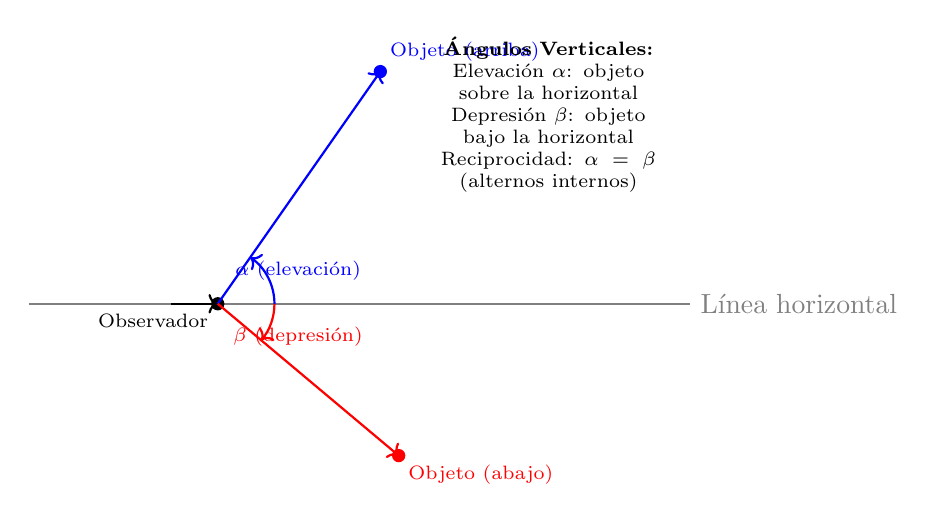
\begin{tikzpicture}[scale=1.2]

  % Línea horizontal de referencia
  \draw[thick, gray] (-2,0) -- (5,0) node[right] {Línea horizontal};
  \draw[->, thick] (-0.5,0) -- (0,0);

  % Observador en el origen
  \fill (0,0) circle (2pt) node[below left] {\scriptsize Observador};

  % Ángulo de elevación (hacia arriba)
  \coordinate (P1) at ({3*cos(55)},{3*sin(55)});
  \draw[blue, thick, ->] (0,0) -- (P1);
  \draw[->, blue, thick] (0.6,0) arc (0:55:0.6);
  \node[blue] at (0.85,0.35) {\scriptsize $\alpha$ (elevación)};

  % Ángulo de depresión (hacia abajo)
  \coordinate (P2) at ({2.5*cos(-40)},{2.5*sin(-40)});
  \draw[red, thick, ->] (0,0) -- (P2);
  \draw[->, red, thick] (0.6,0) arc (0:-40:0.6);
  \node[red] at (0.85,-0.35) {\scriptsize $\beta$ (depresión)};

  % Objetos observados
  \fill[blue] (P1) circle (2pt) node[above right] {\scriptsize Objeto (arriba)};
  \fill[red] (P2) circle (2pt) node[below right] {\scriptsize Objeto (abajo)};

  % Etiquetas de guía
  \node[align=center, text width=4cm, font=\scriptsize] at (3.5, 2) {
    \textbf{Ángulos Verticales:}\\
    Elevación $\alpha$: objeto sobre la horizontal\\
    Depresión $\beta$: objeto bajo la horizontal\\
    Reciprocidad: $\alpha = \beta$ (alternos internos)
  };

\end{tikzpicture}

\end{document}
